\documentclass{standalone}
\usepackage{tikz}
\usetikzlibrary{patterns, positioning}


\begin{document}
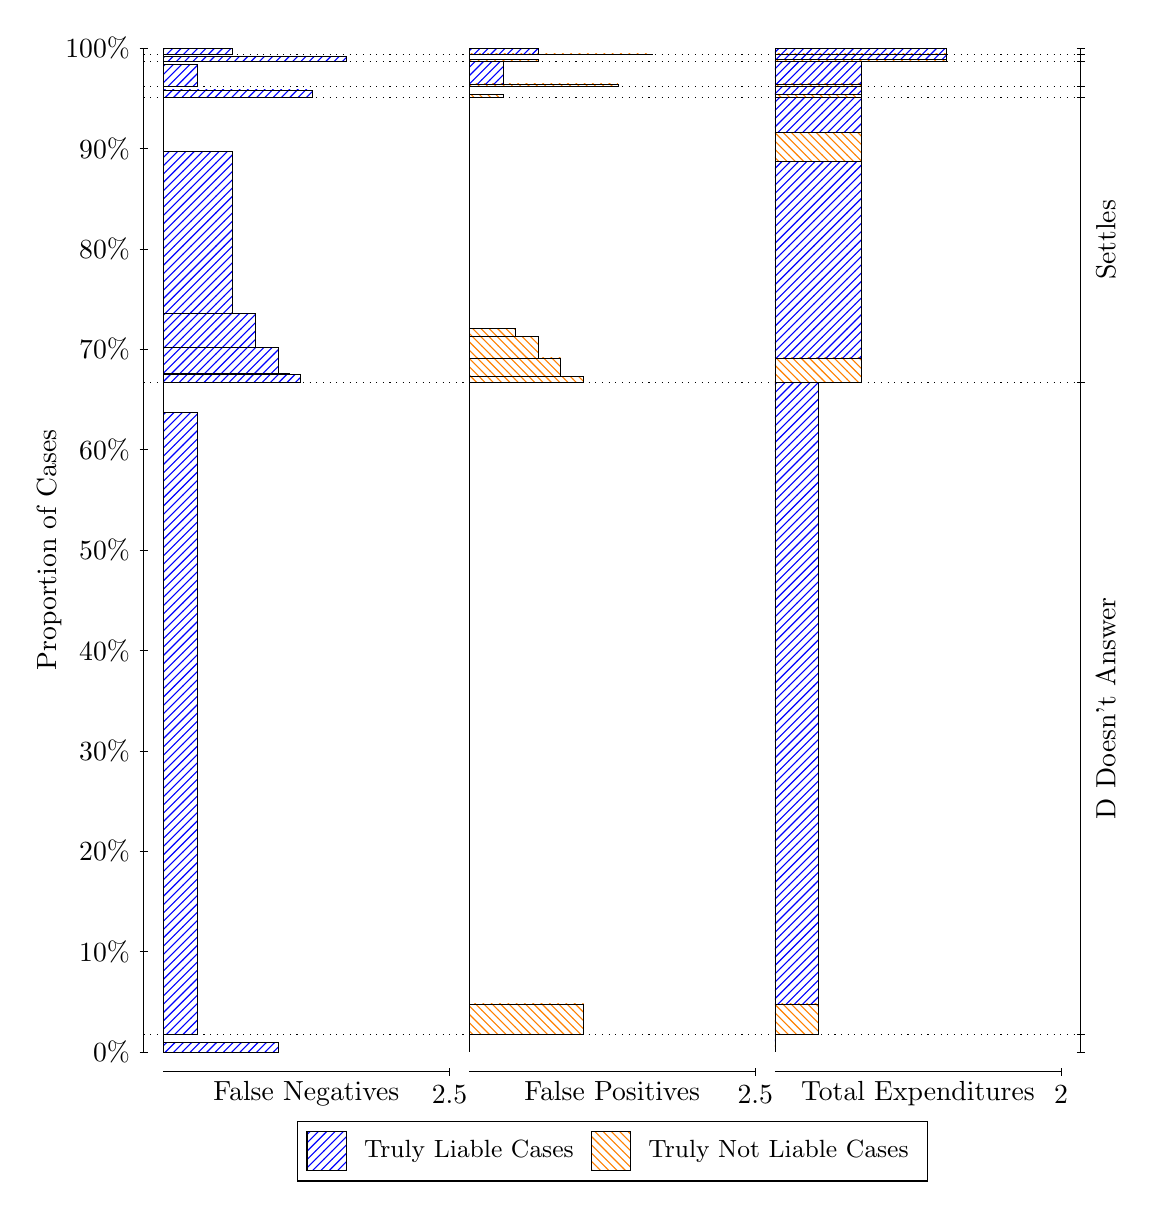
\begin{tikzpicture}
\draw[black, very thin] (1.5,1.75) -- (1.5,14.5);
\node[rotate=90, text=black, anchor=center] at (0.3, 8.125) {Proportion of Cases};
\draw[black, very thin] (1.45,1.75) -- (1.55,1.75);
\node[text=black, anchor=east] at (1.45, 1.75) {0\%};
\draw[black, very thin] (1.45,3.025) -- (1.55,3.025);
\node[text=black, anchor=east] at (1.45, 3.025) {10\%};
\draw[black, very thin] (1.45,4.3) -- (1.55,4.3);
\node[text=black, anchor=east] at (1.45, 4.3) {20\%};
\draw[black, very thin] (1.45,5.575) -- (1.55,5.575);
\node[text=black, anchor=east] at (1.45, 5.575) {30\%};
\draw[black, very thin] (1.45,6.85) -- (1.55,6.85);
\node[text=black, anchor=east] at (1.45, 6.85) {40\%};
\draw[black, very thin] (1.45,8.125) -- (1.55,8.125);
\node[text=black, anchor=east] at (1.45, 8.125) {50\%};
\draw[black, very thin] (1.45,9.4) -- (1.55,9.4);
\node[text=black, anchor=east] at (1.45, 9.4) {60\%};
\draw[black, very thin] (1.45,10.675) -- (1.55,10.675);
\node[text=black, anchor=east] at (1.45, 10.675) {70\%};
\draw[black, very thin] (1.45,11.95) -- (1.55,11.95);
\node[text=black, anchor=east] at (1.45, 11.95) {80\%};
\draw[black, very thin] (1.45,13.225) -- (1.55,13.225);
\node[text=black, anchor=east] at (1.45, 13.225) {90\%};
\draw[black, very thin] (1.45,14.5) -- (1.55,14.5);
\node[text=black, anchor=east] at (1.45, 14.5) {100\%};

\draw[black, very thin] (13.4,1.75) -- (13.4,14.5);
\draw[black, very thin] (13.35,1.75) -- (13.45,1.75);
\node[anchor=west] at (13.35, 1.75) {};
\draw[black, very thin] (13.35,1.9761) -- (13.45,1.9761);
\node[anchor=west] at (13.35, 1.9761) {};
\draw[black, very thin] (13.35,10.256) -- (13.45,10.256);
\node[anchor=west] at (13.35, 10.256) {};
\draw[black, very thin] (13.35,13.869) -- (13.45,13.869);
\node[anchor=west] at (13.35, 13.869) {};
\draw[black, very thin] (13.35,14.011) -- (13.45,14.011);
\node[anchor=west] at (13.35, 14.011) {};
\draw[black, very thin] (13.35,14.326) -- (13.45,14.326);
\node[anchor=west] at (13.35, 14.326) {};
\draw[black, very thin] (13.35,14.418) -- (13.45,14.418);
\node[anchor=west] at (13.35, 14.418) {};
\draw[black, very thin] (13.35,14.5) -- (13.45,14.5);
\node[anchor=west] at (13.35, 14.5) {};

\draw[black, very thin, pattern color=blue, pattern=north east lines] (1.75,1.75) rectangle (3.2033,1.8747);
\draw[black, very thin, pattern color=orange, pattern=north west lines] (1.75,1.8747) rectangle (1.75,1.9761);
\draw[black, very thin, pattern color=blue, pattern=north east lines] (1.75,1.9761) rectangle (2.186,9.873);
\draw[black, very thin, pattern color=orange, pattern=north west lines] (1.75,9.873) rectangle (1.75,10.256);
\draw[black, very thin, pattern color=blue, pattern=north east lines] (1.75,10.256) rectangle (3.494,10.359);
\draw[black, very thin, pattern color=blue, pattern=north east lines] (1.75,10.359) rectangle (3.3487,10.366);
\draw[black, very thin, pattern color=blue, pattern=north east lines] (1.75,10.366) rectangle (3.2033,10.698);
\draw[black, very thin, pattern color=blue, pattern=north east lines] (1.75,10.698) rectangle (2.9127,11.133);
\draw[black, very thin, pattern color=blue, pattern=north east lines] (1.75,11.133) rectangle (2.622,13.189);
\draw[black, very thin, pattern color=orange, pattern=north west lines] (1.75,13.189) rectangle (1.75,13.869);
\draw[black, very thin, pattern color=blue, pattern=north east lines] (1.75,13.869) rectangle (3.6393,13.967);
\draw[black, very thin, pattern color=orange, pattern=north west lines] (1.75,13.967) rectangle (1.75,14.011);
\draw[black, very thin, pattern color=blue, pattern=north east lines] (1.75,14.011) rectangle (2.186,14.292);
\draw[black, very thin, pattern color=orange, pattern=north west lines] (1.75,14.292) rectangle (1.75,14.326);
\draw[black, very thin, pattern color=blue, pattern=north east lines] (1.75,14.326) rectangle (4.0753,14.392);
\draw[black, very thin, pattern color=orange, pattern=north west lines] (1.75,14.392) rectangle (1.75,14.418);
\draw[black, very thin, pattern color=blue, pattern=north east lines] (1.75,14.418) rectangle (2.622,14.493);
\draw[black, very thin, pattern color=orange, pattern=north west lines] (1.75,14.493) rectangle (1.75,14.5);
\draw[black, very thin, pattern color=orange, pattern=north west lines] (5.6333,1.75) rectangle (5.6333,1.8515);
\draw[black, very thin, pattern color=blue, pattern=north east lines] (5.6333,1.8515) rectangle (5.6333,1.9761);
\draw[black, very thin, pattern color=orange, pattern=north west lines] (5.6333,1.9761) rectangle (7.0867,2.3595);
\draw[black, very thin, pattern color=blue, pattern=north east lines] (5.6333,2.3595) rectangle (5.6333,10.256);
\draw[black, very thin, pattern color=orange, pattern=north west lines] (5.6333,10.256) rectangle (7.0867,10.33);
\draw[black, very thin, pattern color=orange, pattern=north west lines] (5.6333,10.33) rectangle (6.796,10.564);
\draw[black, very thin, pattern color=orange, pattern=north west lines] (5.6333,10.564) rectangle (6.5053,10.835);
\draw[black, very thin, pattern color=orange, pattern=north west lines] (5.6333,10.835) rectangle (6.36,10.839);
\draw[black, very thin, pattern color=orange, pattern=north west lines] (5.6333,10.839) rectangle (6.2147,10.936);
\draw[black, very thin, pattern color=blue, pattern=north east lines] (5.6333,10.936) rectangle (5.6333,13.869);
\draw[black, very thin, pattern color=orange, pattern=north west lines] (5.6333,13.869) rectangle (6.0693,13.912);
\draw[black, very thin, pattern color=blue, pattern=north east lines] (5.6333,13.912) rectangle (5.6333,14.011);
\draw[black, very thin, pattern color=orange, pattern=north west lines] (5.6333,14.011) rectangle (7.5227,14.045);
\draw[black, very thin, pattern color=blue, pattern=north east lines] (5.6333,14.045) rectangle (6.0693,14.326);
\draw[black, very thin, pattern color=orange, pattern=north west lines] (5.6333,14.326) rectangle (6.5053,14.352);
\draw[black, very thin, pattern color=blue, pattern=north east lines] (5.6333,14.352) rectangle (5.6333,14.418);
\draw[black, very thin, pattern color=orange, pattern=north west lines] (5.6333,14.418) rectangle (7.9587,14.425);
\draw[black, very thin, pattern color=blue, pattern=north east lines] (5.6333,14.425) rectangle (6.5053,14.5);
\draw[black, very thin, pattern color=orange, pattern=north west lines] (9.5167,1.75) rectangle (9.5167,1.8515);
\draw[black, very thin, pattern color=blue, pattern=north east lines] (9.5167,1.8515) rectangle (9.5167,1.9761);
\draw[black, very thin, pattern color=orange, pattern=north west lines] (9.5167,1.9761) rectangle (10.062,2.3595);
\draw[black, very thin, pattern color=blue, pattern=north east lines] (9.5167,2.3595) rectangle (10.062,10.256);
\draw[black, very thin, pattern color=orange, pattern=north west lines] (9.5167,10.256) rectangle (10.607,10.564);
\draw[black, very thin, pattern color=blue, pattern=north east lines] (9.5167,10.564) rectangle (10.607,13.056);
\draw[black, very thin, pattern color=orange, pattern=north west lines] (9.5167,13.056) rectangle (10.607,13.427);
\draw[black, very thin, pattern color=blue, pattern=north east lines] (9.5167,13.427) rectangle (10.607,13.869);
\draw[black, very thin, pattern color=orange, pattern=north west lines] (9.5167,13.869) rectangle (10.607,13.912);
\draw[black, very thin, pattern color=blue, pattern=north east lines] (9.5167,13.912) rectangle (10.607,14.011);
\draw[black, very thin, pattern color=orange, pattern=north west lines] (9.5167,14.011) rectangle (10.607,14.045);
\draw[black, very thin, pattern color=blue, pattern=north east lines] (9.5167,14.045) rectangle (10.607,14.326);
\draw[black, very thin, pattern color=orange, pattern=north west lines] (9.5167,14.326) rectangle (11.697,14.352);
\draw[black, very thin, pattern color=blue, pattern=north east lines] (9.5167,14.352) rectangle (11.697,14.418);
\draw[black, very thin, pattern color=orange, pattern=north west lines] (9.5167,14.418) rectangle (11.697,14.425);
\draw[black, very thin, pattern color=blue, pattern=north east lines] (9.5167,14.425) rectangle (11.697,14.5);
\draw[black, dotted] (1.5,1.9761) -- (13.4,1.9761);
\draw[black, dotted] (1.5,10.256) -- (13.4,10.256);
\draw[black, dotted] (1.5,13.869) -- (13.4,13.869);
\draw[black, dotted] (1.5,14.011) -- (13.4,14.011);
\draw[black, dotted] (1.5,14.326) -- (13.4,14.326);
\draw[black, dotted] (1.5,14.418) -- (13.4,14.418);
\draw[black, very thin] (1.75,1.5) -- (5.3833,1.5);
\node[text=black, anchor=north] at (3.5667, 1.5) {False Negatives};
\draw[black, very thin] (5.3833,1.45) -- (5.3833,1.55);
\node[text=black, anchor=north] at (5.3833, 1.45) {2.5};

\draw[black, very thin] (5.6333,1.5) -- (9.2667,1.5);
\node[text=black, anchor=north] at (7.45, 1.5) {False Positives};
\draw[black, very thin] (9.2667,1.45) -- (9.2667,1.55);
\node[text=black, anchor=north] at (9.2667, 1.45) {2.5};

\draw[black, very thin] (9.5167,1.5) -- (13.15,1.5);
\node[text=black, anchor=north] at (11.333, 1.5) {Total Expenditures};
\draw[black, very thin] (13.15,1.45) -- (13.15,1.55);
\node[text=black, anchor=north] at (13.15, 1.45) {2};


\node[text=black, centered, rotate=90] at (13.72, 6.1162) {D Doesn't Answer};
\node[text=black, centered, rotate=90] at (13.72, 12.063) {Settles};





\draw (7.449999999999999,1.5) node[draw=none] (baseCoordinate) {};
\begin{scope}[align=center]
        \matrix[scale=0.5, draw=black, below=0.5cm of baseCoordinate, nodes={draw}, column sep=0.1cm]{
            \node[rectangle, draw, minimum width=0.5cm, minimum height=0.5cm, pattern color=blue, pattern=north east lines] {}; &
            \node[draw=none, font=\small, text=black] (B) {Truly Liable Cases}; &
            \node[rectangle, draw, minimum width=0.5cm, minimum height=0.5cm, pattern color=orange, pattern=north west lines] {}; &
            \node[draw=none, font=\small, text=black] (B) {Truly Not Liable Cases}; \\
            };
\end{scope}

\end{tikzpicture}
\end{document}